The discrete time system was implemented with SIMULINK (see figure \ref{fig:modelP13} in Appendix \ref{AppDiscreteTimeP13}) and simulated with the input $u_e(k) = A_u sin(2\pi f_c k T_s)$ and the disturbance vector $\text{d}(k)$ where $k = [0 \ 1 \ ... \ \frac{TIME\_SIM}{STEP\_SIZE} = 50000]$. The results are shown in the time and frequency domains, respectively in figures \ref{fig:P13t} and \ref{fig:P13f} where the responses of P11 are also plotted to allow the comparison. 

In the frequency domain (figure \ref{fig:P13f}), it can be noticed that the amplitudes of the pikes and their positions in the discrete time model perfectly match the ones in continuous time. The discrete time responses are shifted but that does not impact the system since the amplitudes of the harmonics are the same. Moreover, in the time domain (figure \ref{fig:P13t}), the two responses are also similar. For the discrete time system, stairs are visible but since the time is discretised it is expected. It can then be concluded that the simulation results support the sampling time $T_s$ chosen in P12.

\begin{figure}[H]
 \centering 
 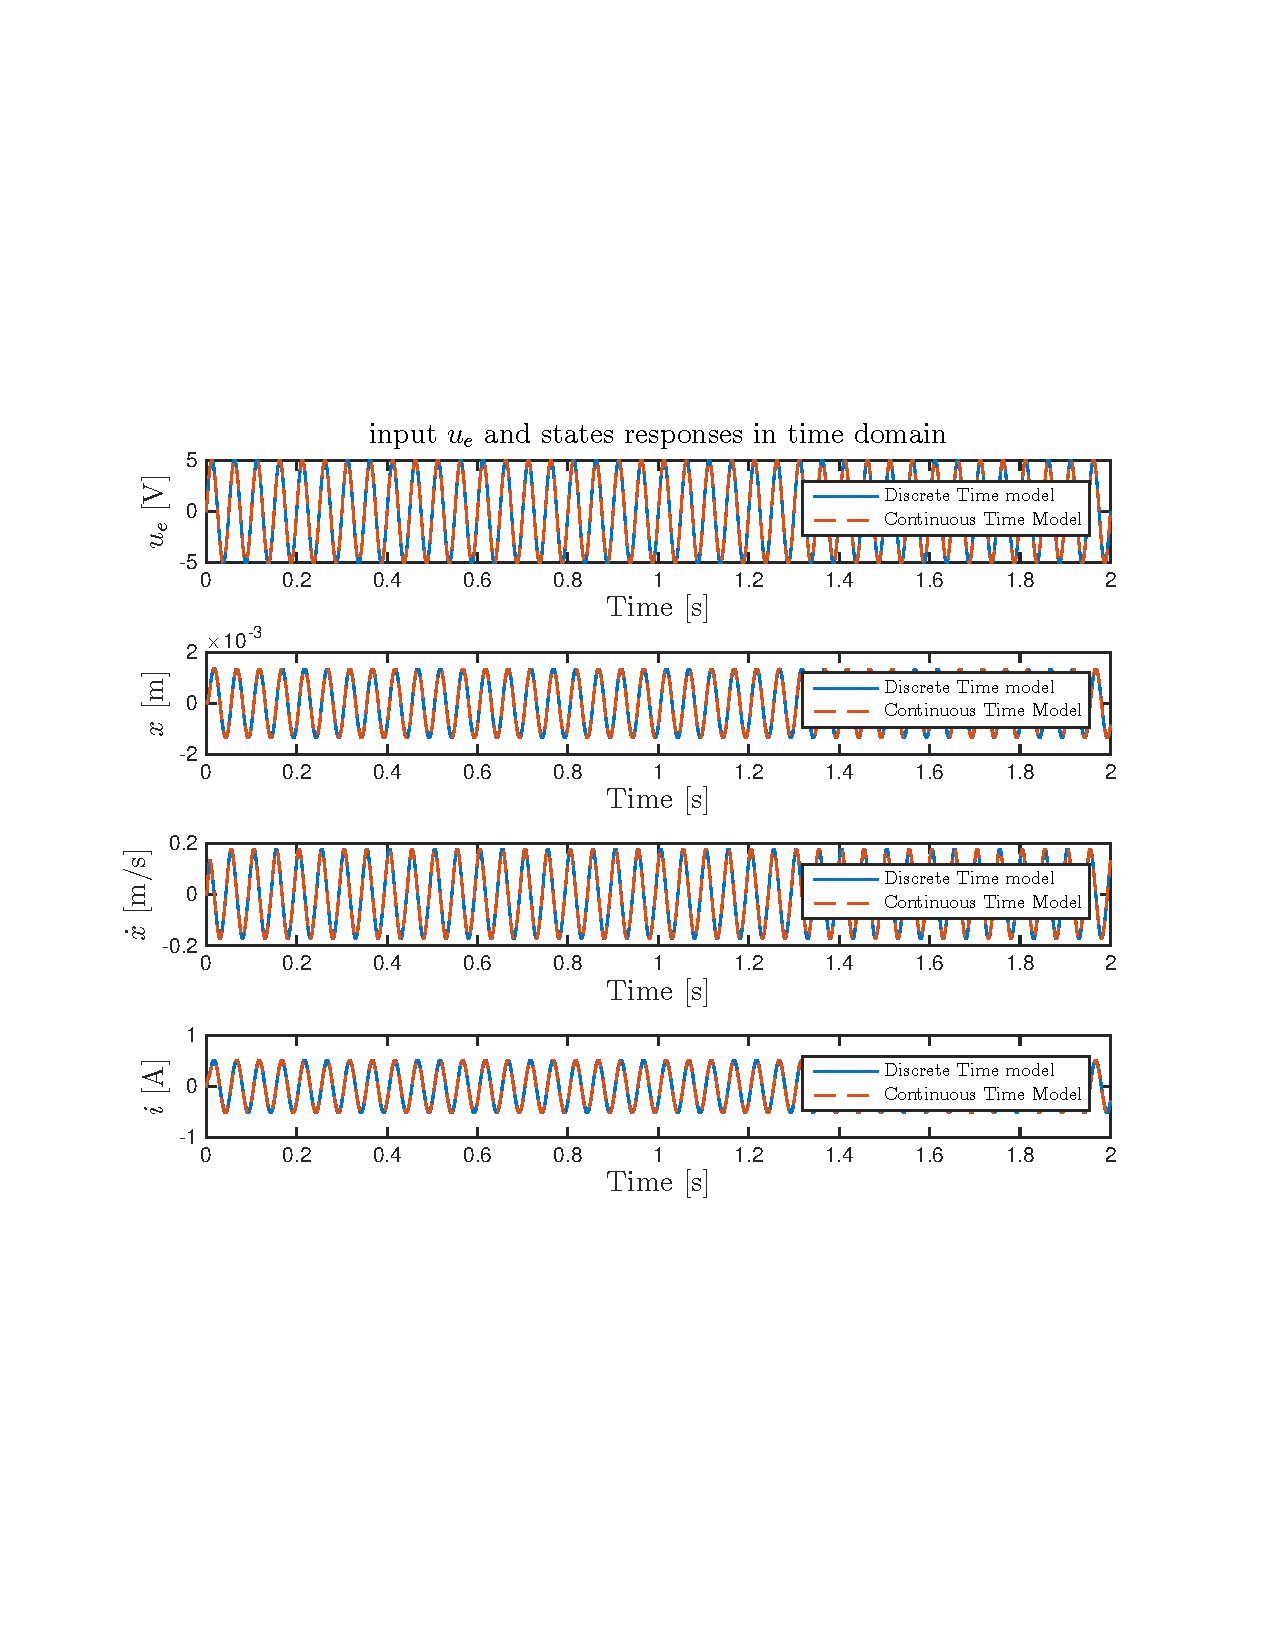
\includegraphics[trim=2cm 7cm 2cm 7cm, clip=true, totalheight=0.35\textheight, angle=0]{figures/P13timeDomain.pdf}
 \caption{Discrete Time Model: input $u_e$ and the states responses in the time domain}
 \label{fig:P13t}
\end{figure}

\begin{figure}[H]
 \centering 
 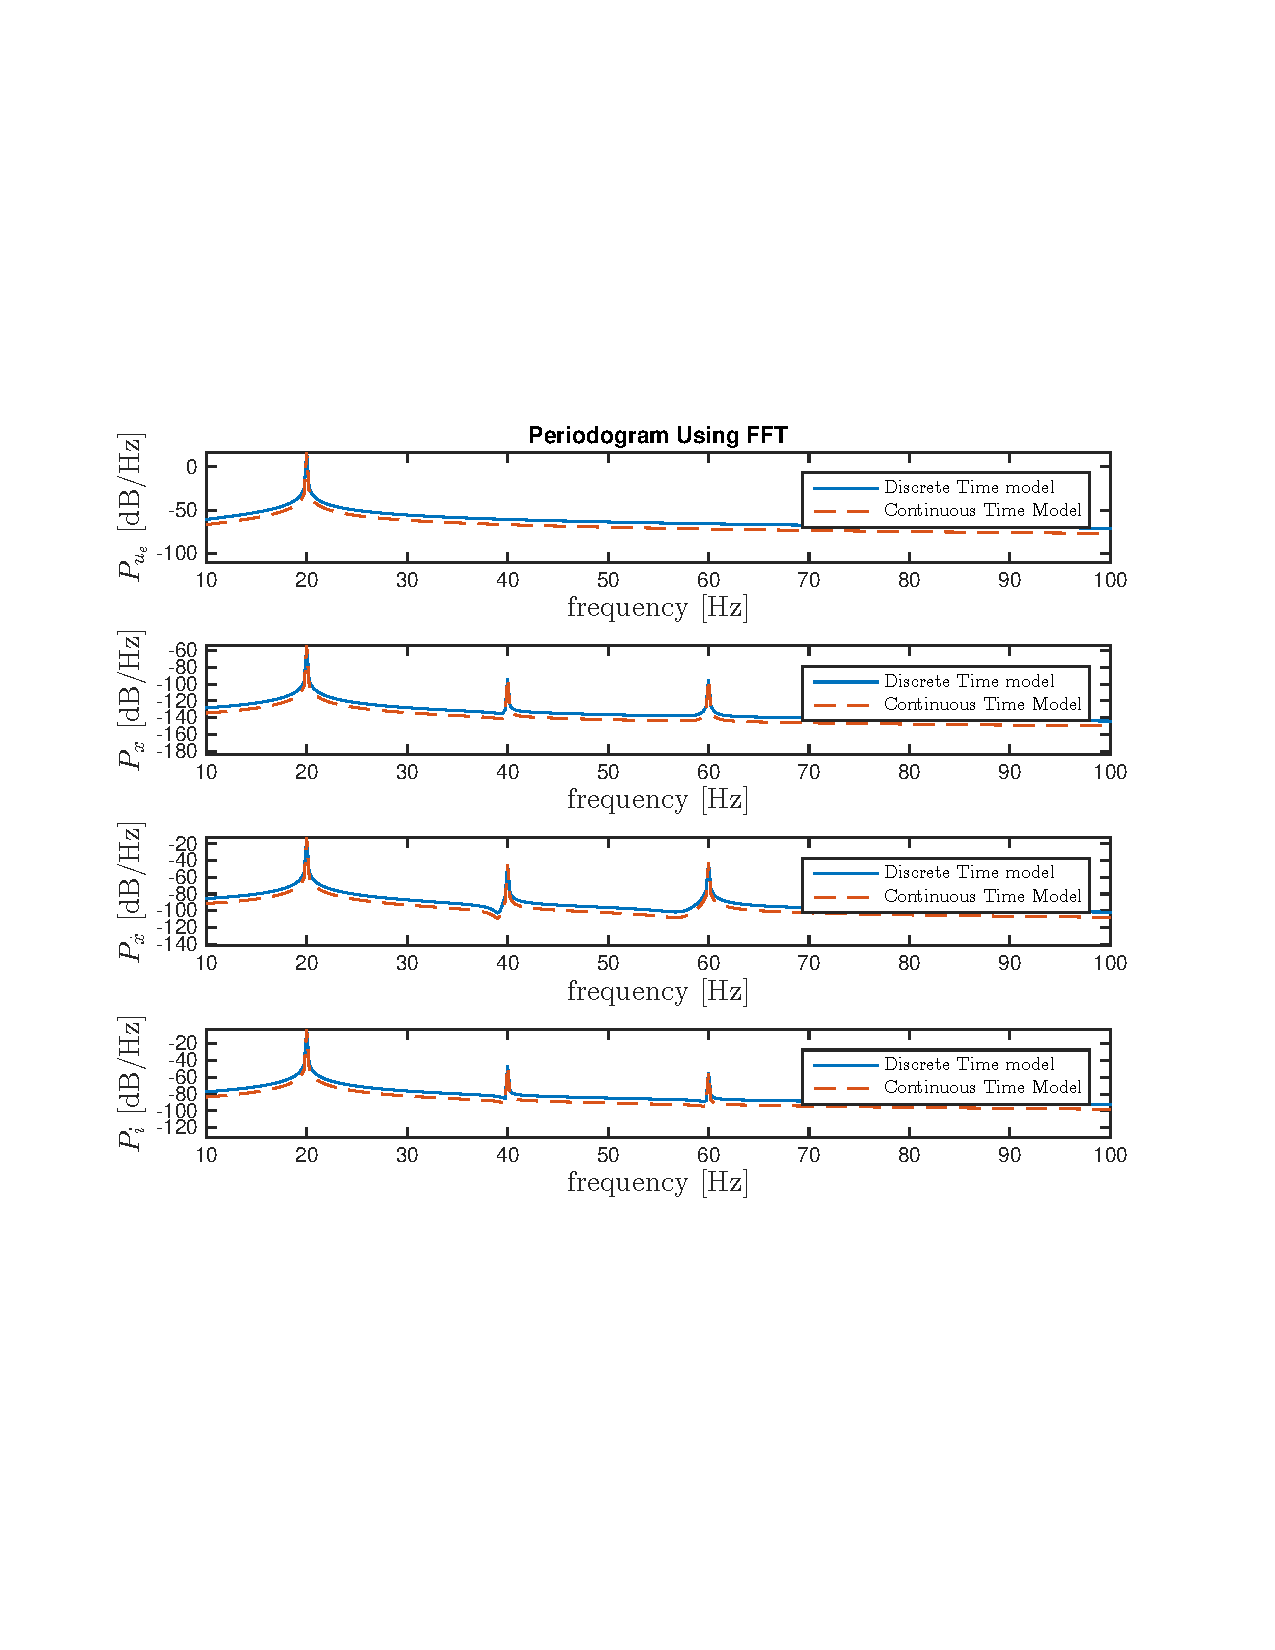
\includegraphics[trim=2cm 7cm 2cm 7cm, clip=true, totalheight=0.35\textheight, angle=0]{figures/P13frequencyDomain.pdf}
 \caption{Discrete Time Model: input $u_e$ and the states responses in the frequency domain}
 \label{fig:P13f}
\end{figure}